\documentclass[11pt]{article}
\usepackage[a4paper,margin=1in]{geometry}
\usepackage[T1]{fontenc}
\usepackage[utf8]{inputenc}
\usepackage{lmodern}
\usepackage{microtype}
\usepackage{booktabs}
\usepackage{enumitem}
\usepackage{graphicx}
\usepackage{hyperref}
\usepackage{xcolor}
\hypersetup{colorlinks=true, linkcolor=black, citecolor=black, urlcolor=blue}

\title{\textbf{Uscha: A Fact-Gated, Tool-Agnostic Methodology for\\Specification-Driven Development with LLM Coding Agents}}
\author{Andr\'es Massello\thanks{This work is licensed under a Creative
Commons Attribution 4.0 International (CC BY 4.0) license.}\\
\small Independent Researcher --- C\'ordoba, Argentina\\
\small \texttt{amassello@gmail.com} $\cdot$ \texttt{github.com/andresmassello}
$\cdot$ \texttt{linkedin.com/in/amassello}}
\date{July 2026}

\begin{document}
\maketitle

\begin{abstract}
LLM coding agents fail in two well-documented ways: when instructions are
underspecified they guess instead of stopping, and when a verification signal is
visible they optimize the signal rather than the requested outcome. We present
\textbf{Uscha}, a methodology for specification-driven development with LLM
coding agents organized around a single discipline: \emph{gates that read facts
block; gates that guess over prose advise}. The methodology contributes (i) two
specification fronts --- a greenfield front where the agent \emph{proposes} the
system shape under one-question-at-a-time human approval, and a brownfield front
where the agent may only \emph{extract} verifiable facts, never author a
specification of existing behavior; (ii) a deterministic evidence ledger with a
two-tier record contract in which measured artifacts always override agent
self-reports; (iii) a family of executable fact gates (golden non-authorship,
gate-integrity, simplicity budgets, per-criterion measured acceptance,
regression capture, a derived --- never self-declared --- workflow state machine)
and a structured-guess layer (versioned qualitative rubrics with mandatory
evidence, and deterministic clone-vs-repository detection that surfaces the
duplication a diff-local simplicity gate cannot see) that advises by default and
gates only by explicit human declaration; and (iv) a strict placement of the
human at three fixed points: approving the shape, approving the golden baseline,
and merging. The methodology also applies its own Lean discipline reflexively:
a meta-invariant that keeps a growing set of good gates from becoming an audit
(over-processing waste), enforced by collapsing every persisted gate into a
single readiness verdict. A reference implementation (seven agent skills and a
dependency-free Python engine with 24 subcommands and adapters for nine language
stacks) is described, together with its design
validation: two adversarial audits (231 agent evaluations) that initially found
the central principle inverted in code and drove its re-wiring; a systematic
cross-examination against classical software-engineering doctrine that produced
ten shipped improvements; and sustained self-application, in which fresh-context
reviews repeatedly caught real defects before merge across the release series. We report design
validation and self-application evidence only; controlled empirical evaluation
remains future work.
\end{abstract}

\section{Introduction}\label{sec:intro}

Two recent empirical results frame the problem this methodology addresses.
First, when task instructions are underspecified, production coding agents do
not fail closed: they act on unstated assumptions, and a majority of runs
violate at least one action boundary~\cite{ji2026guessing}. Second, when a
verification oracle is visible to the agent, near-perfect scores can coexist
with an undelivered artifact: the agent \emph{builds to the test}, optimizing
the check rather than the request, and does not on its own validate what it
ships as a user would~\cite{ma2026building}. Both failures are dispositional
rather than capability failures, and both worsen as agents are given more
autonomy.

Existing agent development frameworks converge on persistent artifacts and
human review as mitigations~\cite{demacedo2026prompt}, but they largely encode
their process as \emph{prose instructions that the agent may ignore}, and their
verification signals rarely distinguish between what is mechanically verifiable
and what is a model's opinion. Uscha\footnote{``Uscha'' is the name of the
methodology; the pattern it operationalizes is a \emph{spec-loop} --- a
specification-driven build-and-verify loop.} starts from that distinction and
makes it the organizing principle of the whole process. Figure~\ref{fig:system}
shows the resulting pipeline: eight stations from idea to human gate, under a
constitution of invariants that no station may violate, with an inner
convergence loop over the build and an outer proposal loop that returns to
discovery --- while the merge remains human.

\begin{figure}[t]
\centering
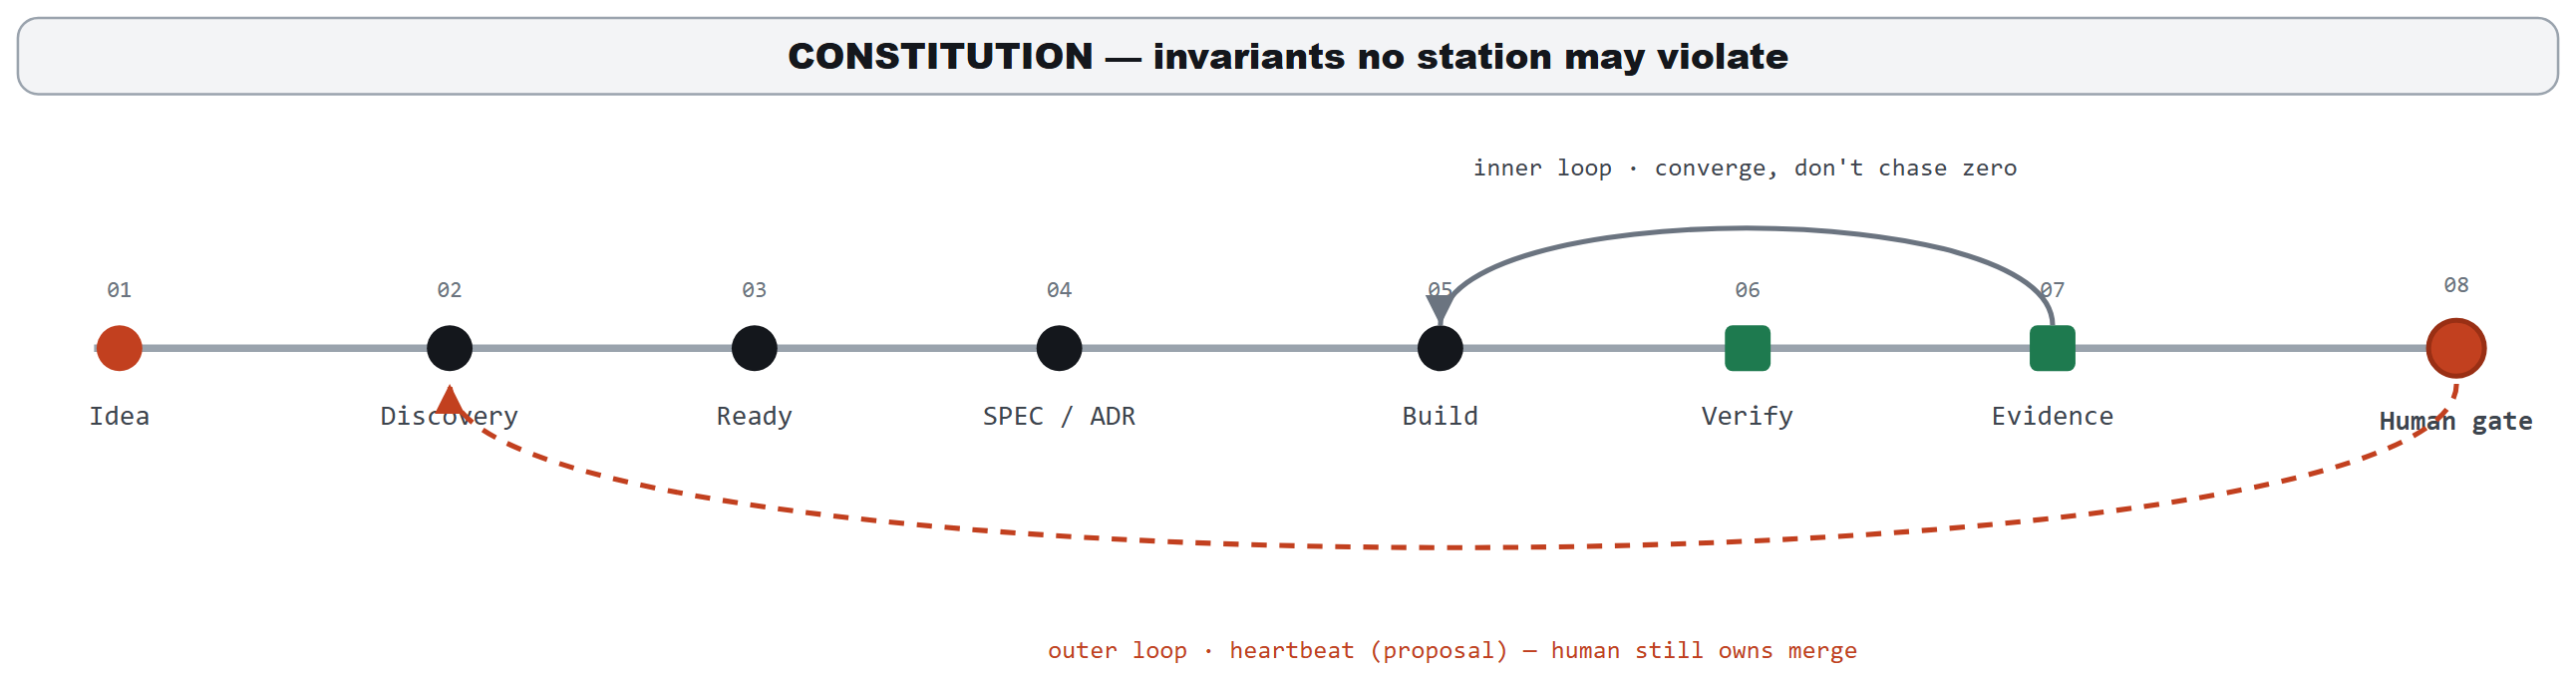
\includegraphics[width=\linewidth]{fig1-system-map.png}
\caption{The Uscha pipeline. Eight stations from idea to human gate under
a constitution of inviolable invariants. The inner loop
(build--verify--evidence) converges instead of chasing zero findings; the
outer loop returns evidence to discovery as a proposal --- the human still
owns the merge.}
\label{fig:system}
\end{figure}

The methodology is built on one discipline and three architectural commitments:

\begin{description}[leftmargin=1.2em]
\item[Facts block; guesses advise.] Every check in the process is classified as
\emph{computational} (it reads an artifact --- a byte comparison, a parsed test
report, a diff structure) or \emph{inferential} (it judges prose or code
quality). Computational checks are allowed to block progress mechanically.
Inferential checks may only advise, unless a human explicitly declares them
gating. A natural-language heuristic that blocks produces false positives, gets
disabled, and dies; keeping guesses advisory is what keeps them alive.
\item[Measured beats narrated.] The evidence ledger records two tiers: measured
records parsed from real artifacts (test reports, coverage files, linter
output) and self-reported agent counts. A measured red always overrides a
narrated green. Acceptance criteria close per criterion only when a green,
name-tagged test case exists in the ingested reports --- a checked checkbox
without a test is recorded as \emph{narrated-only} and does not close.
\item[The human at three fixed points.] The human approves the \emph{shape}
(specification front), approves the \emph{golden baseline} (the one artifact
the agent is mechanically forbidden from authoring), and \emph{merges}. The
agent proposes, measures, and stops.
\item[Tool-agnosticism by contract.] The engine is dependency-free Python that
never runs an LLM: it validates structures and ingests reports. Wherever a
model's judgment participates (e.g.\ rubric grading), the interface is a JSON
contract; who produced the JSON --- one vendor's agent, another's, or a human
--- is irrelevant to the ledger.
\end{description}

This paper describes the methodology (\S\ref{sec:method}), its evidence engine
(\S\ref{sec:engine}), the reference implementation (\S\ref{sec:impl}), and the
design-validation evidence accumulated so far (\S\ref{sec:validation}),
followed by limitations (\S\ref{sec:limitations}) and future work
(\S\ref{sec:future}).

\section{Related Work}\label{sec:related}

\textbf{Underspecification.} Ji et al.~\cite{ji2026guessing} show that
underspecified operational instructions cause agents to guess rather than
stop, violating action boundaries in 55.8--67.8\% of runs. Uscha's
greenfield front is a direct response: the specification is produced through a
structured interrogation in which the agent proposes and the human decides,
and inviolable constraints are captured in a constitution file whose breach is
a first-class blocker, never a trade-off.

\textbf{Building to the test.} Ma et al.~\cite{ma2026building} demonstrate
that agents deliver what is checked, not what is requested, and name the
missing disposition \emph{validation self-awareness}. Uscha treats this as
its central adversary: acceptance closes per criterion on measured test
evidence; findings cannot be closed without new test material (\emph{find bugs
once}); qualitative verdicts require file-and-line evidence or they do not
count; and the workflow state that authorizes a pull request is derived from
ledger facts, never self-declared by the agent.

\textbf{Process taxonomies.} de Macedo~\cite{demacedo2026prompt} surveys agent
development frameworks along six dimensions (specification, context, roles,
execution, validation, portability) and identifies recurring risks:
specification drift, artifact fragility, and platform dependence. Uscha
addresses each explicitly: drift through a rebuild test that scores whether
the specification package alone can regenerate the system; fragility through
an integrity-checksummed ledger; and platform dependence through the contract
architecture and a dependency-free engine.

\textbf{Practitioner doctrine.} The methodology's check classification adapts
the computational-versus-inferential distinction from B\"ockeler's
\emph{sensor} framework for coding agents~\cite{boeckeler2025sensors,fowler2023exploring}
--- the axis on which ``facts block, guesses advise'' rests. Its gate-integrity
stance --- that a change must not weaken the apparatus that measures it, and
that a high-blast-radius change needs a checker uncorrelated with the maker ---
follows the agentic-code-review red flags catalogued by Osmani~\cite{osmani2025agentic}.
Architecture decision records follow Nygard~\cite{nygard2011adr}, extended with
machine-checkable implementation plans. Golden-master capture follows
approval-testing practice~\cite{approvaltests}, with one addition central to the
method: the agent may author the capture harness but is mechanically forbidden
--- by a pre-tool-use hook, not by instruction --- from writing an approved
fixture. The simplicity gate operationalizes the ``Reduce'' law of
Maeda~\cite{maeda2006simplicity}. The methodology was also systematically
cross-examined against classical
doctrine~\cite{thomas2019pragmatic}; \S\ref{sec:validation} reports the ten
resulting improvements. Two agent-native failure modes complete the lineage:
the premature ``done'' token --- Huntley's \emph{Ralph Wiggum
loop}~\cite{huntley2025ralph} --- is exactly what the derived state machine and
objective gates refuse to accept, and the maker-checker separation the review
loop enforces is the evaluator-optimizer pattern~\cite{anthropic2024agents}.
The design stance throughout is an application of Goodhart's
law~\cite{strathern1997improving} to agent verification: any signal the agent
can see, it will eventually optimize.

\section{The Methodology}\label{sec:method}

\subsection{Two specification fronts}

\textbf{Greenfield (discovery).} The human brings an idea; the agent brings
the \emph{shape}. The front proceeds one question at a time, each question
carrying the agent's recommended answer, walking a fixed agenda: purpose,
domain model, operation surface, architecture options with trade-offs, dirty
cases and failure behavior, inviolable constraints, out-of-scope, acceptance
criteria with stable traceable identifiers, a declared quality bar, and
residual risks. High-uncertainty risks trigger a time-boxed \emph{spike} whose
only legitimate output is a decision record with lessons --- spike branches are
mechanically refused at the pull-request gate. The front emits a versioned
specification package: context glossary, constitution, domain model,
specification, decision records with implementation plans and verification
checklists, acceptance file, risks, and handoff. Figure~\ref{fig:hierarchy}
shows how the package's artifacts feed the evidence engine and how the engine
verifies the result across six layers of truth.

\begin{figure}[t]
\centering
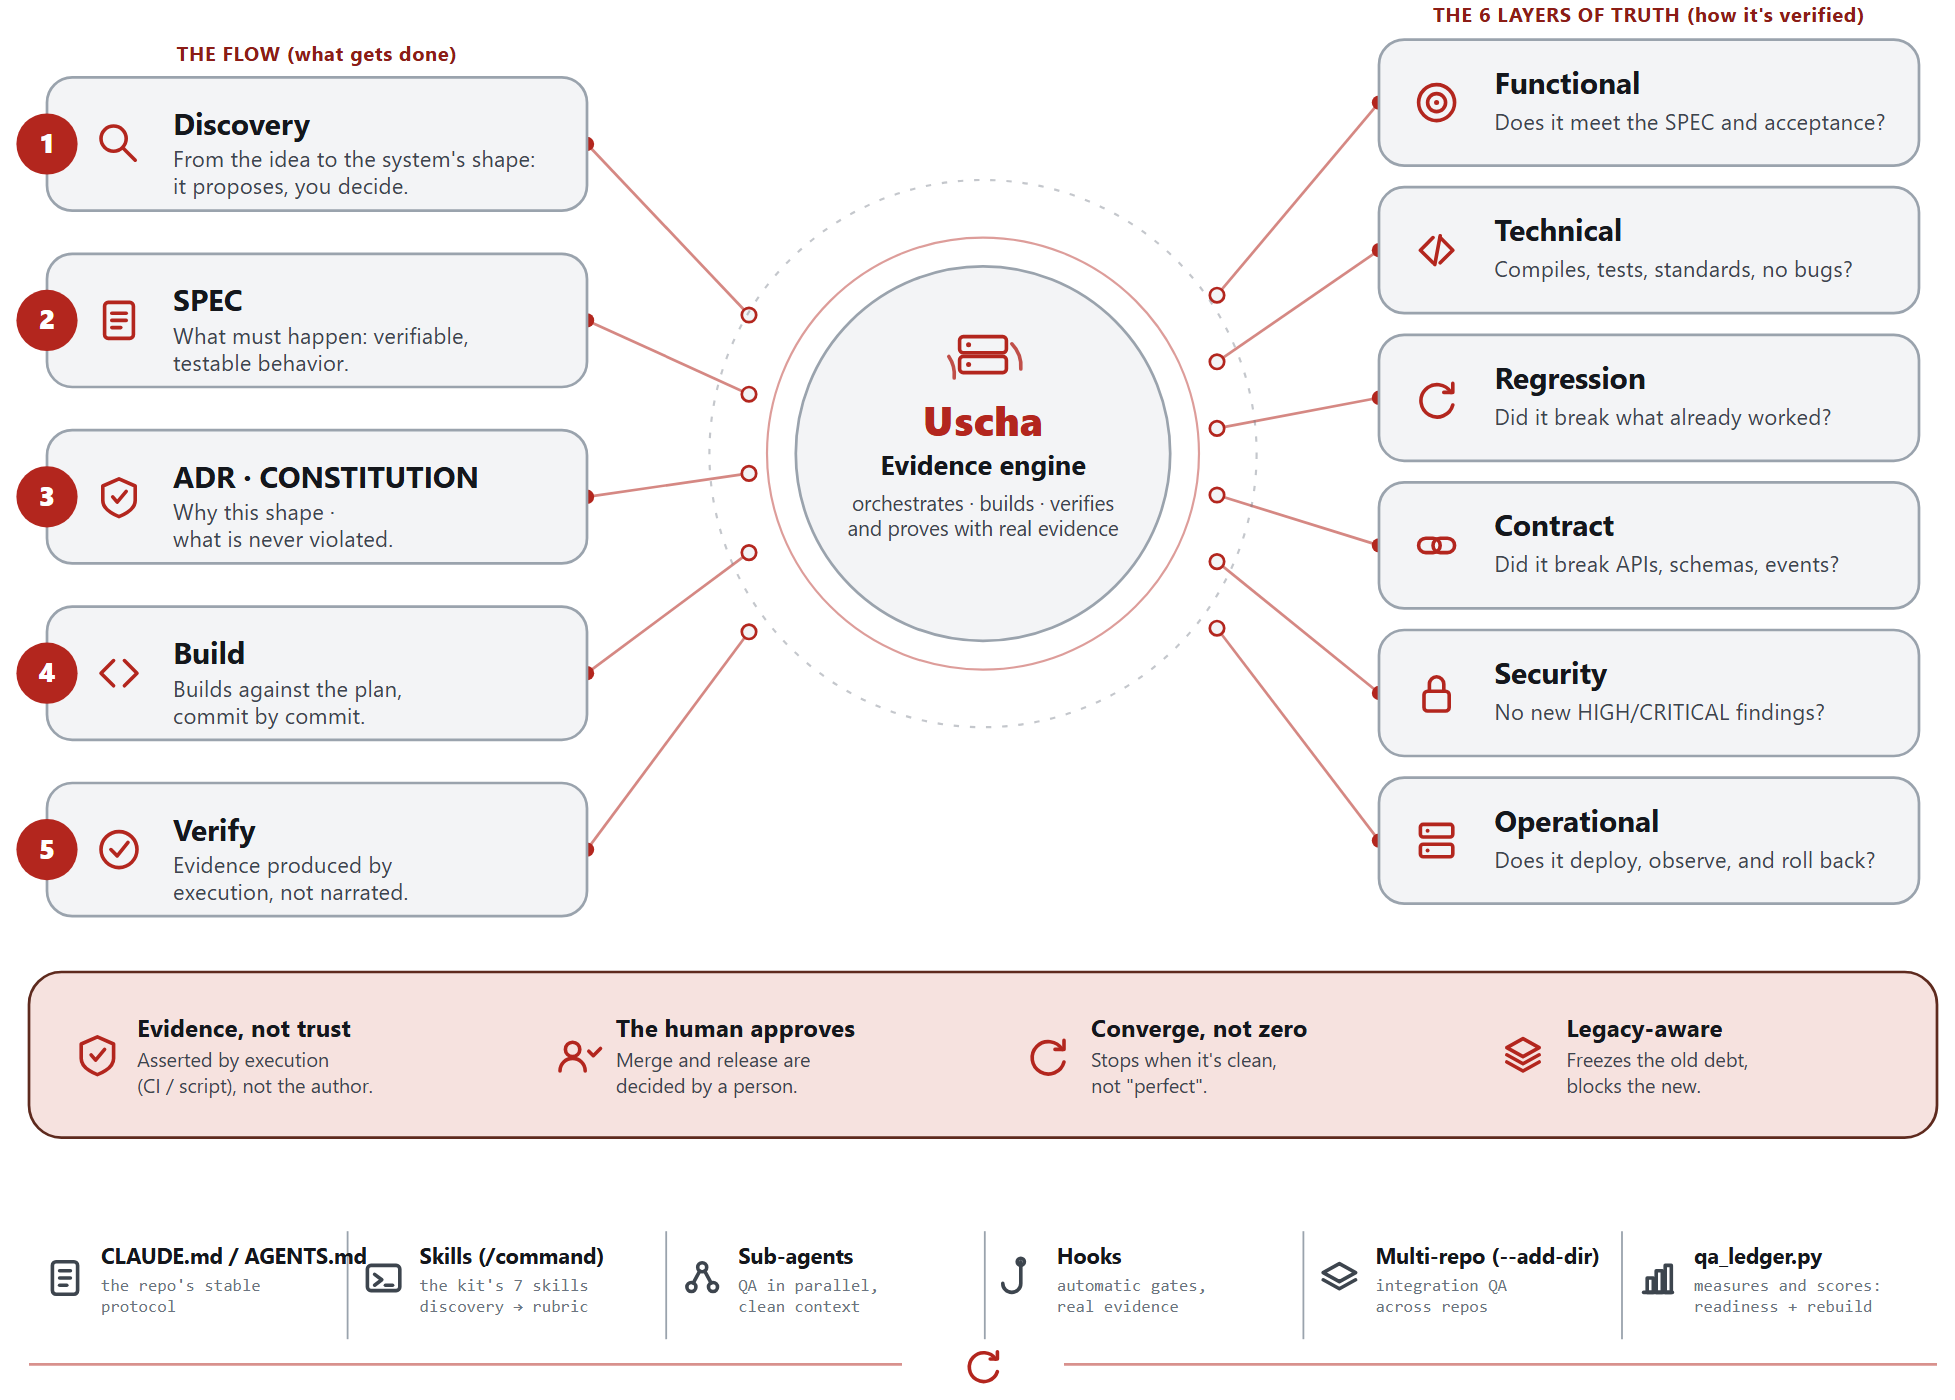
\includegraphics[width=\linewidth]{fig2-spec-hierarchy.png}
\caption{The specification package (left: what gets done) and the six layers
of truth (right: how it is verified), joined by the evidence engine. The
bottom band states the four commitments the diagram encodes: evidence produced
by execution rather than asserted by the author; merge and release decided by
a person; convergence instead of perfection; and legacy awareness --- freeze
the old debt, block the new.}
\label{fig:hierarchy}
\end{figure}

\textbf{Brownfield (reverse discovery).} For an existing system, the direction
of trust inverts: observable behavior is ground truth, and the agent may
produce \emph{only facts} --- a system map from static analysis and a golden
suite captured mechanically at the boundaries. The agent never authors a
specification of what the old system does or why: a specification written by
the agent about legacy code encodes the same partial reading of the code that
loses behavior silently, which is precisely the blind spot the golden exists
to counter. The human writes the migration specification by reading the facts.

\subsection{The development loop}

The loop consumes the specification package and proceeds through phases, each
guarded: plan (constitution first; no acceptance criteria, no build); a
coverage gate that triggers boundary characterization tests when the safety
net is insufficient; build under decision-record discipline (the agent
consults records before touching governed areas and must propose --- never
silently take --- new architectural decisions); a simplicity gate scoring the
diff against declared budgets, with test code excluded so that writing tests
is never penalized; a severity-gated review loop that \emph{converges instead
of chasing zero} (findings below the declared gate are deferred, not fixed
forever); an integration pass across repositories; late test-writing against
stabilized code; an optional rebuild test measuring specification
completeness; and a pull request opened only when the derived workflow state
says the facts allow it. The loop stops at merge: merging is human.

An escalation contract enumerates the situations in which the agent must stop
and ask --- iteration cap, oscillating findings, a previously-passing test now
failing non-trivially, contradictory tool directives, decisions of
architectural weight, and any constitution breach. Escalations and their
closures are recorded events; an open escalation caps the readiness score
until a human resolves it, and resolving a blocker requires an \emph{escape
analysis}: which gate or test should have caught this, and what was done about
it.

\subsection{A worked example in ten steps}

Figure~\ref{fig:tensteps} walks a deliberately small feature --- a discount
calculation --- through the whole methodology, because the small case makes
the failure modes legible. Six of the ten steps are failures or refinements,
and that is the point: each deviation is caught by a specific gate rather than
by hope. Two advisory passes tighten the specification before any code exists
(a vague criterion becomes a testable oracle; a missing out-of-scope section
is added). During the build, mutation testing exposes a test that runs but
asserts nothing (\emph{coverage was lying}); the gate-integrity check catches
and blocks the agent lowering a threshold to pass; the rebuild test diverges
on an implicit input case, and the response is to amend the specification,
never the code; the simplicity gate cuts a speculative abstraction. Only then
does the readiness score --- capped by facts, dominated by measured acceptance
--- reach the human gate, where a person reads the diff and approves the
merge.

\begin{figure}[t]
\centering
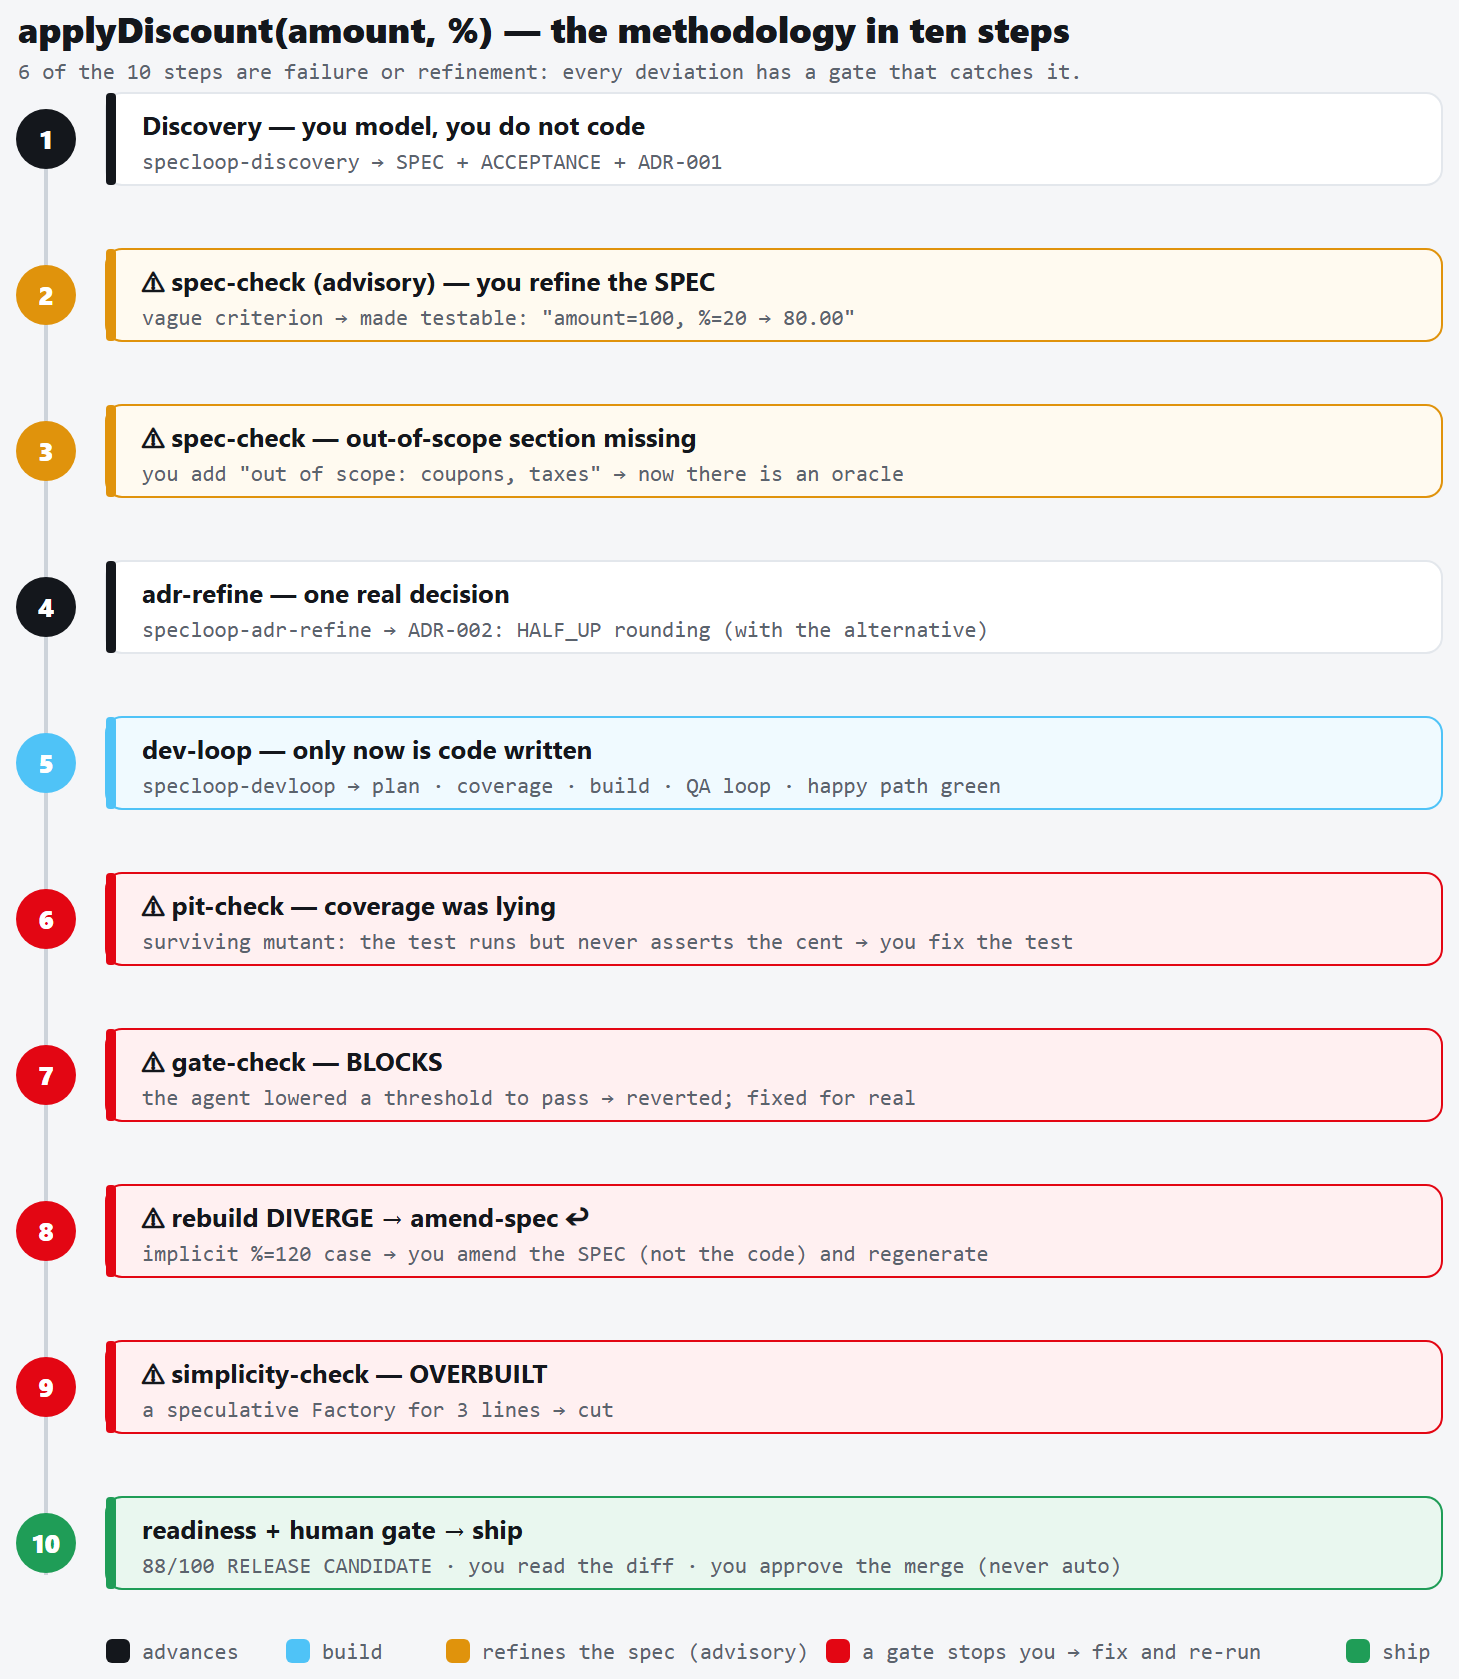
\includegraphics[width=0.78\linewidth]{fig3-ten-steps.png}
\caption{A worked example: \texttt{applyDiscount(amount,~\%)} through the ten
steps of the methodology. Black steps advance (blue marks the build), amber
steps refine the specification (advisory), red steps are gates stopping the
agent (fix and re-run), and the final green step is the human gate. Six of ten steps being
failure or refinement is the expected shape of the process, not an anomaly.}
\label{fig:tensteps}
\end{figure}

\section{The Evidence Engine}\label{sec:engine}

The engine is a single dependency-free Python file. It never runs an LLM and
never runs the tools it scores: it \emph{ingests} their reports (JUnit-family
XML, Cobertura and lcov coverage, nine linter formats across nine language
stacks) and validates structures. Every verdict is persisted in a
deterministic ledger with an integrity checksum; external mutation or a
truncated write blocks loading with a recovery message.
Table~\ref{tab:checks} summarizes the complete check family and the verdict
class of each.

\begin{table}[t]
\centering
\small
\begin{tabular}{@{}lp{8.6cm}l@{}}
\toprule
\textbf{Check} & \textbf{Reads} & \textbf{Verdict} \\
\midrule
\texttt{golden-diff} & byte comparison against human-approved fixtures;
declared volatiles masked \emph{visibly} & blocks \\
\texttt{gate-check} & diff structure: deleted/disabled tests (nine stack
conventions), lowered thresholds, added secrets & blocks \\
\texttt{pit-check} & mutation-testing reports (test effectiveness, because
coverage lies) & blocks \\
\texttt{simplicity-check} & diff size, nesting, net growth against declared
budgets; test code excluded & blocks \\
\texttt{spec-check} (structure) & missing sections, zero traceable acceptance
identifiers, duplicates, invalid rubric structure & blocks \\
\texttt{phase --require pr-ready} & workflow state derived from ledger facts;
spike branches always refused & blocks \\
\texttt{readiness} & weighted state score with hard caps and threshold
provenance & reports \\
\texttt{regression-check} & findings closed without new non-blank test lines
$\rightarrow$ narrated closure & advises* \\
\texttt{rubric-ingest} & weighted qualitative criteria; evidence-or-nothing
grader contract & advises* \\
\texttt{waste-check} & Type-1/2 clone windows of the diff vs the repository ---
the duplication a diff-local gate cannot see & advises* \\
\texttt{spec-check} (prose) & vagueness and shape heuristics over
specification text & advises* \\
\bottomrule
\end{tabular}
\caption{The check family. Verdicts marked * advise by default and gate only
under explicit human declaration (configuration or flag); the declaration is
surfaced everywhere as \emph{requirement (declared)} versus \emph{default (kit
opinion)}.}
\label{tab:checks}
\end{table}

\textbf{Fact gates (block).} The blocking gates read artifacts, not opinions.
Two design choices deserve emphasis. First, the golden gate's masking of
volatile fields (timestamps, request identifiers) is itself governed: masking
rules are declared in a versioned file that the human approves together with
the fixtures, every masked match is reported separately, and any later edit to
the rules file is flagged --- masking is never invisible. Second, the workflow
state machine is \emph{derived}: the state (plan, build, qa, escalated,
pr-ready) is computed from ledger facts. A self-declared state machine would
be narrated state --- the exact category of signal the methodology distrusts
--- so there is nothing to declare and no illegal transition to police.

\textbf{Structured guesses (advise).} The advisory layer includes regression
capture (closing findings without adding a single non-blank test line is
flagged as \emph{narrated closure}; the failing test goes before the fix);
plateau and stop-signal advisories over the finding history (findings flat or
rising across three complete cycles means more iteration is not approaching
the solution --- return to the decision records; everything converged with
zero blocking facts means cut and ship); and the rubric layer: a versioned
file of weighted qualitative criteria --- conventions, error-handling sanity,
interface ergonomics, documentation quality --- with anchor examples, negative
criteria, and a threshold, graded by any runner against a JSON contract with
evidence-or-nothing semantics: a verdict that affects the score without a
file-and-line citation does not count, duplicate verdicts for one criterion
break the contract, and unevaluated criteria count as failed (unevaluated is
not approved). The advisory layer also carries \emph{reuse detection}: a
deterministic Type-1/Type-2 clone check of the diff against the existing
repository. This targets the duplication that a diff-local simplicity gate is
blind to by construction --- the muda most characteristic of generated
code~\cite{poppendieck2006lean,gitclear2026gap}. It too reports a fact (a
byte-identical window already exists at \texttt{file:line}) while leaving the
verdict ``wasteful'' advisory, because a normalized-line proxy has honest false
positives (boilerplate, data-transfer objects, embedded SQL) and a check that
blocks on those would be disabled and die.

\textbf{Readiness and the anti-ceremony invariant.} A weighted 0--100 score
reports the state of the result, never effort (Table~\ref{tab:readiness}). The
dominant dimension is measured acceptance --- criteria closed by green,
name-tagged tests --- with checkbox completion demoted to a narrative
dimension. Hard caps override the weighted average, and every biting threshold
states its provenance. The score reports; it does not gate --- the gates are
the facts above. As the gate set grows, the dominant risk shifts from any one
bad gate to the \emph{sum} of good ones making the loop feel like an audit ---
over-processing, the ceremony form of waste. The methodology answers this
reflexively with a meta-invariant every future gate must satisfy (it runs
without human input, speaks only when it matters, collapses into readiness, and
a trivial change skips it), mechanized as a single-verdict view: readiness
collapses every persisted gate into one line, expandable on demand. This is the
same Lean lens the method applies to code, turned on the method
itself~\cite{poppendieck2006lean}.

\begin{table}[t]
\centering
\small
\begin{tabular}{@{}lcp{8.6cm}@{}}
\toprule
\textbf{Dimension} & \textbf{Weight} & \textbf{Measured from} \\
\midrule
acceptance (measured) & 30 & criteria closed by green, name-tagged test cases
in ingested reports \\
static gate & 20 & latest linter runs, normalized severities; never-ran scores
0 (silence is not success) \\
\texttt{adr} (narrative completion) & 15 & checkbox ratio of the acceptance
file --- narrated progress, deliberately demoted below measured acceptance \\
coverage & 15 & coverage reports against the declared threshold \\
convergence & 10 & clean last cycle of every review tool plus clean persisted
fact gates \\
integration & 10 & cross-repository contract pass (weight redistributed if
disabled) \\
\bottomrule
\end{tabular}
\caption{Readiness dimensions and default weights. Hard caps override the
average: red tests $\le$35, open blocker/critical findings $\le$65, unresolved
escalation $\le$75 --- each cap reporting whether its threshold is a declared
requirement or a kit default.}
\label{tab:readiness}
\end{table}

\section{Reference Implementation}\label{sec:impl}

The reference implementation packages the methodology as seven agent skills
(the two fronts, a precision interview for known features, the loop
orchestrator, golden capture, a two-audience system-documentation generator,
and the rubric grader adapter) plus the engine (24 subcommands). Three
properties matter for portability. First, the skills are markdown instruction
files readable by any instruction-following agent; the engine is invoked
identically from any of them. Second, every LLM-judgment interface is a
contract: the rubric grader ships as a neutral prompt usable by any vendor's
agent, a raw API call, or a human filling the JSON by hand --- the
implementation's test suite exercises exactly that path, with no LLM in the
loop. Third, the one mechanical prohibition (the agent must not write approved
golden fixtures) is enforced by a pre-tool-use hook at the runtime boundary,
not by instruction --- during development of the implementation itself the hook
blocked one of its author's own commands, which is the property working as
designed. Table~\ref{tab:skills} maps the seven skills to the phase each serves.

\begin{table}[t]
\centering
\small
\begin{tabular}{@{}llp{6.4cm}@{}}
\toprule
\textbf{Skill} & \textbf{Front / phase} & \textbf{Role} \\
\midrule
\texttt{discovery} & greenfield front & idea $\to$ spec package, one question
at a time; the agent \emph{proposes} the system shape \\
\texttt{adr-refine} & known-feature front & Socratic interview $\to$ SPEC +
decision records + acceptance for an already-scoped feature \\
\texttt{reverse-discovery} & brownfield front & extract \emph{facts} only
(system map + boundary golden); never authors an inferred spec \\
\texttt{characterize} & pre-change & capture the approval suite of current
behavior --- the one artifact the agent must not author \\
\texttt{devloop} & the loop & plan $\to$ build $\to$ severity-gated review loop
$\to$ derived PR gate; records every step in the ledger \\
\texttt{sysdoc} & reporting & two-audience (commercial + technical) HTML deck
generated from the ledger \\
\texttt{rubric} & advisory gate & thin adapter that grades against a versioned
\texttt{RUBRIC.md} via the vendor-neutral JSON contract \\
\bottomrule
\end{tabular}
\caption{The seven agent skills. Each is a markdown instruction file readable by
any instruction-following agent; the engine is invoked identically from each.}
\label{tab:skills}
\end{table}

The implementation carries its process in executable form. A smoke suite of
161 checks exercises the engine against a synthetic ledger --- including,
deliberately, the agnosticism claim: the rubric-layer tests fill the grader's
JSON by hand, with no model in the loop. The engine also reports a passive Lean
process metric --- first-time yield, the fraction of repositories that cleared
QA on the first cycle with no rework or escalation --- derived from ledger facts
and kept strictly informational, never a gate: it measures the process, not the
state of the result. Version consistency across the five
release artifacts (version file, configuration, changelog, plugin manifest,
marketplace manifest) is itself a suite check, converting a release convention
into a verifiable fact. An installation-diagnosis subcommand in the spirit of
\texttt{flutter doctor} verifies interpreter, per-stack toolchains, hook
presence and registration, skill integrity, and per-project configuration ---
and every failing check carries its remedy (an installation link or command),
so the workflow is: run, install what is listed, re-run until green. Three
installation modes are supported: per-project, per-user, and as a packaged
plugin for one agent runtime --- packaging, not dependency; the other runtimes
install by copying files.

\section{Design Validation and Self-Application}\label{sec:validation}

No controlled external evaluation has been conducted yet; we report the
design-validation evidence honestly and completely.

\textbf{Adversarial audits.} Before stabilization, the methodology and its
implementation were subjected to two adversarial audits totaling 231 agent
evaluations: a seven-lens audit (54 agents; findings attacked by skeptics
defaulting to \emph{refuted}) confirmed 33 weaknesses and refuted 13, with the
central finding that the core principle was \emph{inverted in the code} ---
fact gates existed but were not wired to block. A second audit verified 171
claims across documentation, code, and design intent. The response re-wired
every fact gate into the engine and re-passed all documentation against the
implemented reality (a recorded truth-pass over the affected documents),
converting the principle from slogan to enforced property.

\textbf{Doctrine cross-examination.} The methodology was systematically read
against classical software-engineering doctrine~\cite{thomas2019pragmatic},
producing 8 validations, 12 tensions with recorded resolutions, and 10
actionable improvements --- all ten implemented, each as a separate release
with its own regression checks. The validations were often word-for-word:
``don't assume it --- prove it'' is the ledger's two-tier contract; shared
mutable resources including \emph{files} motivated the ledger's integrity
checksum; and the doctrine's warning against trusting enforcement to good
intentions is exactly why the golden prohibition is a hook rather than an
instruction. In the two deepest tensions the methodology
deliberately departed from the letter of the doctrine to defend its own
principle: readiness caps continue to bite by default (their existence is a
definition; only the numbers are opinion, and they now state their
provenance), and the workflow state machine is derived rather than declared.

\textbf{Self-application.} The implementation is developed under its own
process. Across the eighteen releases of the self-application arc (versions
1.10 through 1.27), each engine change carried smoke checks in the same commit,
a fresh-context review before merge, and a five-way version consistency check
enforced by the suite. These reviews repeatedly caught real defects prior to
merge --- the changelogs record the resulting hardening across the series ---
including: test-file
classifier gaps that made a documented guarantee an overclaim; a blank-line
loophole in regression-capture evidence (any non-blank test line counts as
evidence --- a tripwire, not a judge --- but a blank line must not); a
review-suite check that passed for the wrong reason (its precondition never
held, so the assertion was vacuous); silent last-wins semantics on
duplicated grader verdicts --- a grader gaming vector, now a broken-contract
error; and, in the single-verdict release itself, documentation that
under-enumerated what the collapsed view actually shows. We take the
consistency of this defect stream as evidence for the methodology's core
premise: independent, fresh-context checking against recorded criteria
catches what the authoring context cannot see.

\section{Limitations and Threats to Validity}\label{sec:limitations}

\textbf{No controlled evaluation.} All evidence is design validation and
self-application by the methodology's author; effect sizes on team
productivity, defect escape rates, or comparison against the frameworks
surveyed in~\cite{demacedo2026prompt} are unmeasured.
\textbf{Single-operator bias.} Self-application shares authorship context;
although reviews run in fresh contexts, they share the model family and the
author's configuration.
\textbf{LLM non-determinism.} The rubric layer's grades vary across runs;
the methodology bounds the blast radius (advisory by default,
evidence-or-nothing, human-declared gating) but does not eliminate variance.
\textbf{Scope.} The loop targets a single operator driving one non-trivial
change; multi-operator concurrency is out of scope, and the ledger is
single-writer by design.
\textbf{Heuristic residue.} Some gates carry documented approximations
(path-based test classification, stale-report windows); each is disclosed at
the point of use, but disclosure is not elimination.

\section{Future Work}\label{sec:future}

The central gap is controlled evaluation. Concretely, we plan a study that
assigns matched non-trivial changes to operators \emph{with} and \emph{without}
the methodology and measures three outcomes the ledger already instruments:
defect-escape rate at human review, rework (first-time yield across cycles),
and time-to-merge --- against two baselines, ad-hoc agent use and the
frameworks surveyed in~\cite{demacedo2026prompt} along their six taxonomy
dimensions (with particular attention to the validation and portability axes).
The missing pieces are operators other than the author and a controlled task
set; the process instrumentation is already in place. Supporting steps:
read-only dry runs of all nine stack adapters against real repositories; a
multi-project dogfooding phase; and an evaluation of the rubric layer's
inter-run variance under anchored versus unanchored criteria, connecting to the
validation self-awareness agenda of~\cite{ma2026building}. A further direction extends the Lean lens beyond the
inner loop: the reuse and anti-ceremony gates address two forms of waste
(duplication and over-processing), but the ``shine'' discipline of 5S ---
scheduled cleanup that keeps the legacy layer from silently freezing --- is a
candidate \emph{outer-loop} routine~\cite{poppendieck2006lean}, deliberately
out of scope here because it acts on the repository over time rather than on a
single change under review.

\section{Conclusion}\label{sec:conclusion}

Uscha's contribution is not a new agent architecture but a discipline for
placing trust: facts block, guesses advise, the measured overrides the
narrated, and the human decides at exactly three points. The methodology's own
history --- a central principle found inverted by adversarial audit, then
wired into an engine that now blocks its own author when he crosses the line
--- suggests that for LLM-assisted development, the difference between a
methodology and a slogan is whether the checks are executable. The reference
implementation will be released as open source (MIT).

\begin{thebibliography}{9}

\bibitem{ji2026guessing}
Z.~Ji, Z.~Zhang, C.~Xu, Z.~Li, Y.~Gao, S.~Wang, and S.-C.~Cheung,
``Coding Agents Are Guessing: Measuring Action-Boundary Violations in
Underspecified DevOps Instructions,'' arXiv:2607.02294 [cs.SE], 2026.

\bibitem{ma2026building}
Y.~Ma, B.~Kereopa-Yorke, and B.~Schultz,
``Building to the Test: Coding Agents Deliver What You Check, Not What You
Requested,'' arXiv:2606.28430 [cs.SE], 2026.

\bibitem{demacedo2026prompt}
S.~Oliveira de Macedo,
``From Prompt to Process: a Process Taxonomy and Comparative Assessment of
Frameworks Supporting AI Software Development Agents,''
arXiv:2606.04967 [cs.SE], 2026.

\bibitem{thomas2019pragmatic}
D.~Thomas and A.~Hunt,
\emph{The Pragmatic Programmer: Your Journey to Mastery}, 20th Anniversary
Edition. Addison-Wesley, 2019.

\bibitem{nygard2011adr}
M.~Nygard, ``Documenting Architecture Decisions,'' blog post, 2011.
\url{https://cognitect.com/blog/2011/11/15/documenting-architecture-decisions}

\bibitem{boeckeler2025sensors}
B.~B\"ockeler, ``Maintainability Sensors for Coding Agents,''
martinfowler.com, 2025.
\url{https://martinfowler.com/articles/sensors-for-coding-agents.html}

\bibitem{osmani2025agentic}
A.~Osmani, ``Agentic Code Review'' and ``Loop Engineering,'' addyosmani.com,
2024--2025.

\bibitem{maeda2006simplicity}
J.~Maeda, \emph{The Laws of Simplicity}. MIT Press, 2006.

\bibitem{huntley2025ralph}
G.~Huntley, ``The Ralph Wiggum Loop,'' blog post, 2025.

\bibitem{anthropic2024agents}
Anthropic, ``Building Effective Agents'' (the evaluator-optimizer workflow),
2024. \url{https://www.anthropic.com/research/building-effective-agents}

\bibitem{fowler2023exploring}
M.~Fowler et al., ``Exploring Generative AI,'' memo series,
martinfowler.com, 2023--2026.
\url{https://martinfowler.com/articles/exploring-gen-ai.html}

\bibitem{approvaltests}
L.~Falco et al., ``ApprovalTests,'' \url{https://approvaltests.com}.

\bibitem{strathern1997improving}
M.~Strathern, ``\,`Improving ratings': audit in the British University
system,'' \emph{European Review}, vol.~5, no.~3, pp.~305--321, 1997.

\bibitem{poppendieck2006lean}
M.~Poppendieck and T.~Poppendieck, \emph{Implementing Lean Software
Development: From Concept to Cash}. Addison-Wesley, 2006.

\bibitem{gitclear2026gap}
GitClear, ``AI Copilot Code Quality / The Maintainability Gap,'' industry
research report, 2024--2026. \url{https://www.gitclear.com}

\end{thebibliography}

\end{document}
